\section{Results}
\label{sec:results}
\para{Main outcomes.} \Tabref{tab:main-accuracy} shows that self-critique performs worst among full-set conditions. Accuracy drops from 0.3958 to 0.1667 (\decrease), while re-decoding also drops to 0.2500. The external-critique subset reaches 0.2500 and does not recover baseline subset performance.

\begin{table}[t]
\centering
\caption{Condition-level accuracy on the 48-example evaluation set. Best result is bolded.}
\label{tab:main-accuracy}
\begin{tabular}{@{}lc@{}}
\toprule
Condition & Accuracy \\
\midrule
Baseline & {\bf 0.3958} \\
Re-decode control & 0.2500 \\
Self-critique revised & 0.1667 \\
External-critique revised (subset, $n{=}16$) & 0.2500 \\
\bottomrule
\end{tabular}
\end{table}


\para{Dataset-level behavior.} \Tabref{tab:dataset-accuracy} shows that baseline performance is carried mainly by CommonsenseQA (0.7917), where both second-pass conditions degrade strongly. GSM8K is near-floor for baseline and re-decode, with a small absolute increase under self-critique (0.0833), but this does not offset the larger CSQA degradation.

\begin{table}[t]
\centering
\caption{Dataset-wise accuracy by condition. Best value in each row is bolded.}
\label{tab:dataset-accuracy}
\begin{tabular}{@{}lccc@{}}
\toprule
Dataset & Baseline & Re-decode & Self-critique \\
\midrule
\textsc{CommonsenseQA} ($n{=}24$) & {\bf 0.7917} & 0.5000 & 0.2500 \\
\textsc{GSM8K} ($n{=}24$) & 0.0000 & 0.0000 & {\bf 0.0833} \\
\bottomrule
\end{tabular}
\end{table}


\para{Paired significance and transitions.} Self-critique causes a significant paired drop (McNemar $p=0.0098$). Transition counts from baseline to self-revised are 2 improved, 13 degraded, and 33 unchanged, confirming that harmful revisions dominate.

\begin{table}[t]
\centering
\caption{Key statistical tests comparing reflection conditions against baseline or control.}
\label{tab:stats}
\begin{tabular}{@{}ll@{}}
\toprule
Metric & Value \\
\midrule
Self - Baseline delta & $-0.2292$ (95\% CI: $[-0.3750,-0.0625]$) \\
Re-decode - Baseline delta & $-0.1458$ (95\% CI: $[-0.2708,-0.0208]$) \\
McNemar $p$ (Self vs Baseline) & 0.0098 \\
Mean cosine drift (Self) & 0.5700 \\
Mean cosine drift (Re-decode) & 0.5719 \\
Paired Wilcoxon $p$ (mean drift, Self vs Re-decode) & 0.7643 \\
Layer-wise FDR-significant differences (28 tests) & 0 \\
\bottomrule
\end{tabular}
\end{table}


\para{Representation drift.} \Figref{fig:drift} plots per-layer cosine drift profiles. Self-critique and re-decode curves closely overlap across layers, and no layer remains significant after FDR correction (28 tests). On per-example mean drift, paired Wilcoxon $p=0.7643$, consistent with no measurable critique-specific increase in drift magnitude.

\begin{figure}[t]
    \centering
    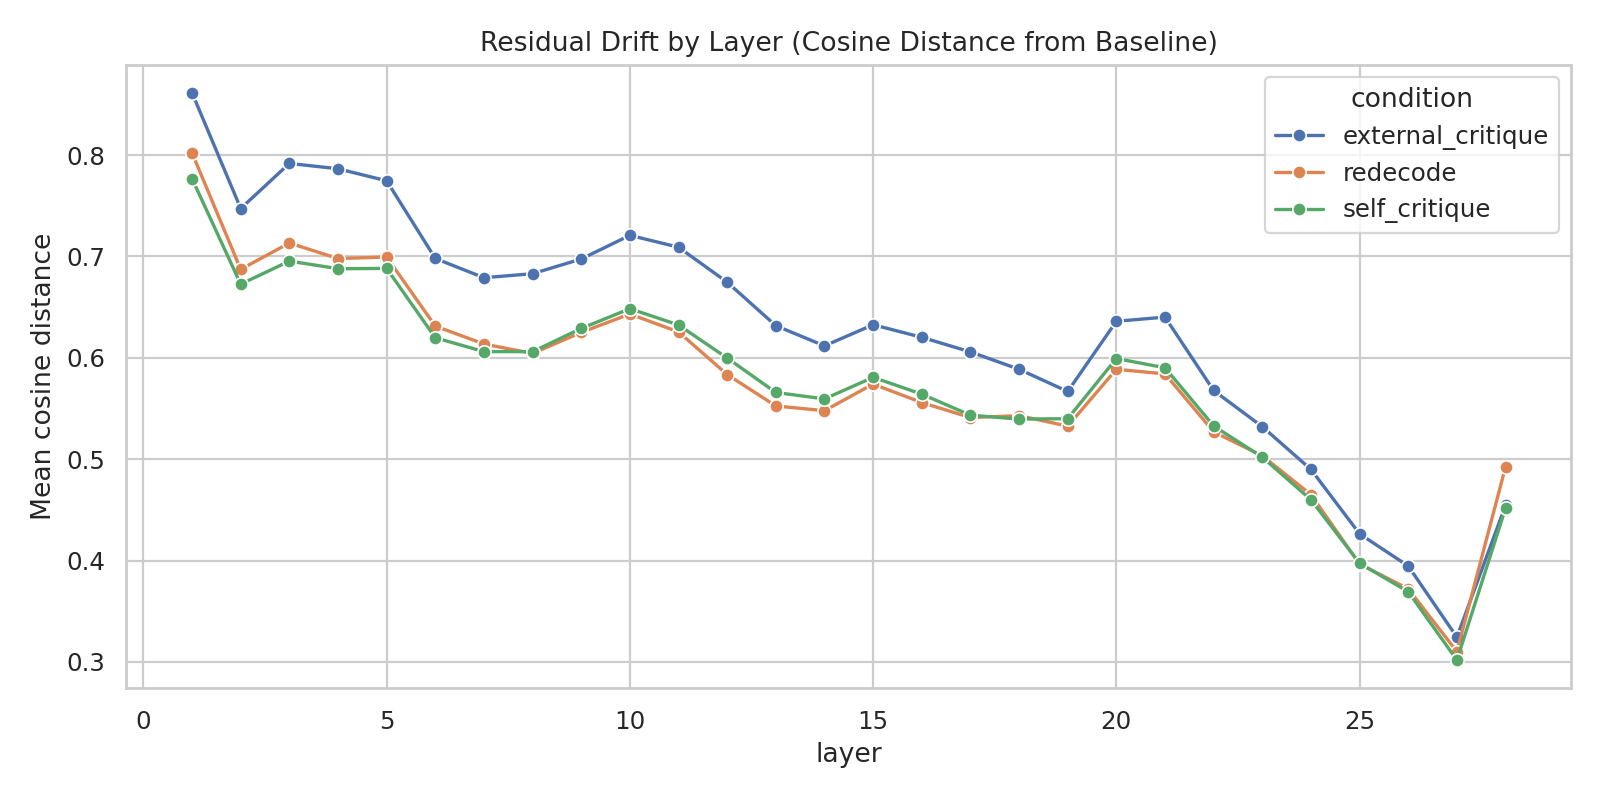
\includegraphics[width=0.95\linewidth]{figures/drift_by_layer.png}
    \caption{Layer-wise cosine drift from baseline hidden states. Self-critique and re-decode have highly similar profiles across all 28 layers, with no FDR-significant layer-wise difference.}
    \label{fig:drift}
\end{figure}

\para{Accuracy and correction visuals.} \Figref{fig:accuracy} summarizes condition-level accuracy, and \figref{fig:corrections} shows sparse correction outcomes among initially wrong examples.

\begin{figure}[t]
    \centering
    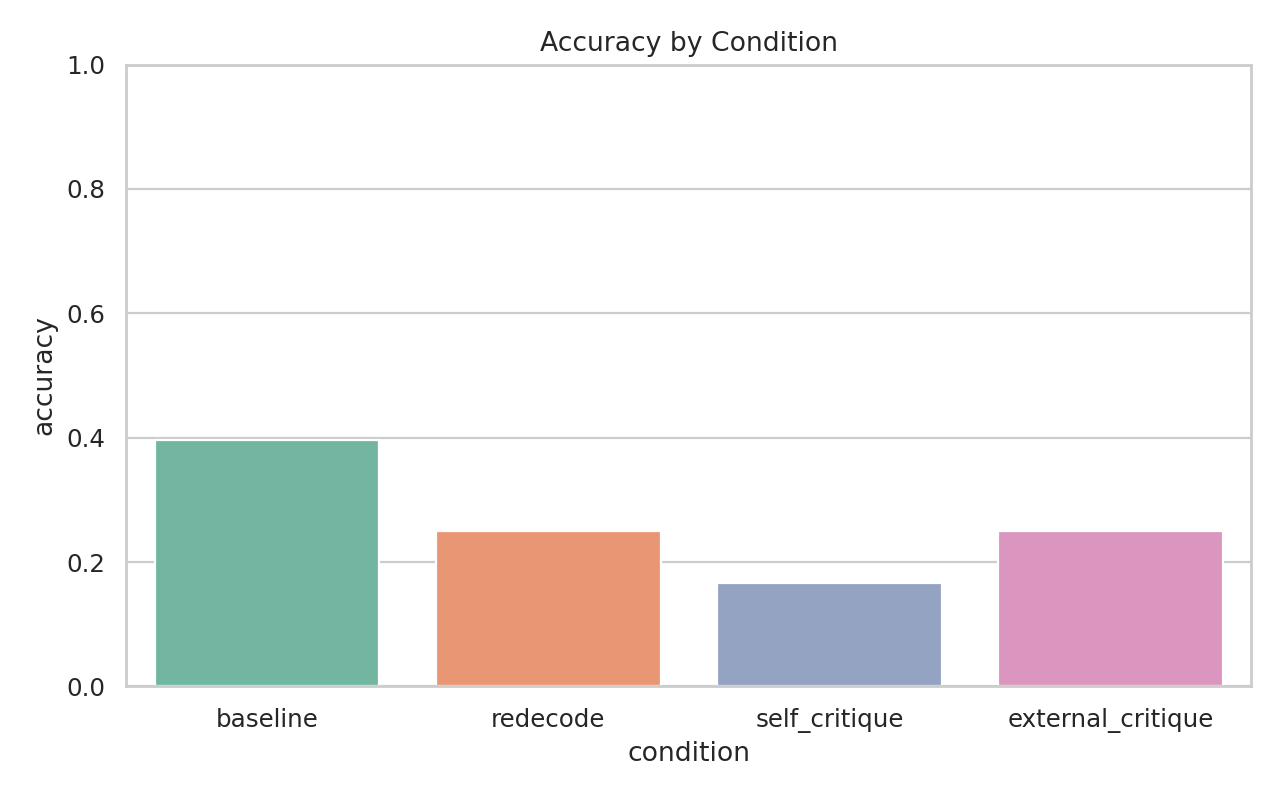
\includegraphics[width=0.95\linewidth]{figures/accuracy_by_condition.png}
    \caption{Accuracy by condition. Both second-pass strategies reduce performance relative to one-shot baseline, with the largest drop under intrinsic self-critique.}
    \label{fig:accuracy}
\end{figure}

\begin{figure}[t]
    \centering
    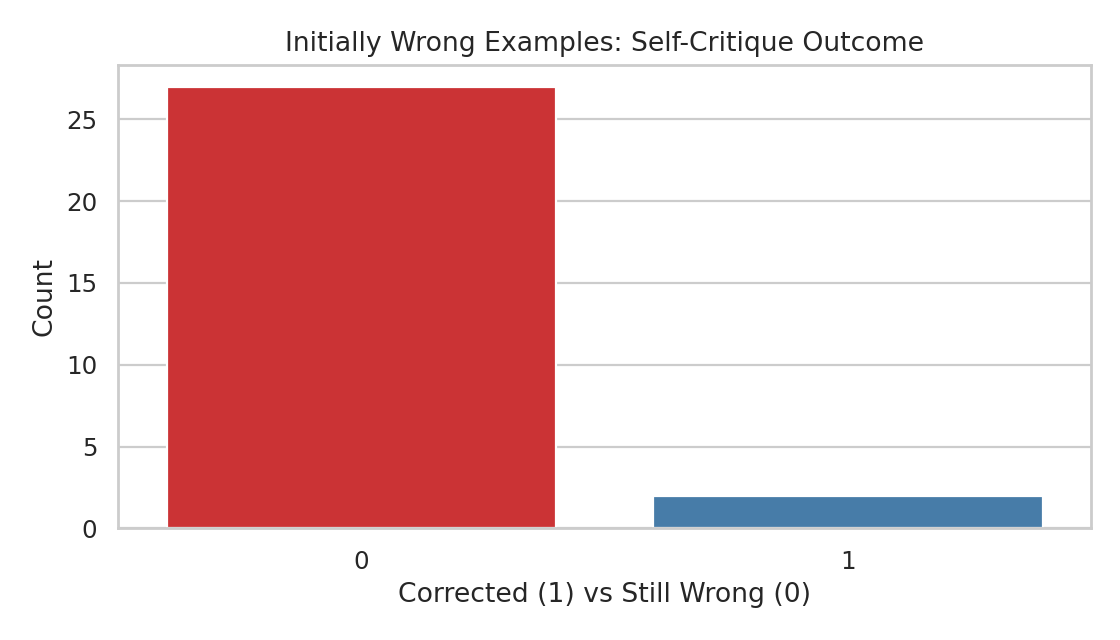
\includegraphics[width=0.95\linewidth]{figures/correction_outcomes.png}
    \caption{Correction outcomes for self-critique transitions. Only two initially wrong examples are corrected, while many initially correct cases degrade.}
    \label{fig:corrections}
\end{figure}

\para{Probe separability.} Probe evaluation is underpowered: only 2/29 positives (6.9\%) among initially wrong examples. Several folds produce undefined AUC, and mean F1 is 0.0. We therefore avoid strong claims about separability in this run.
